\chapter{Probabilistic modeling of team coordination}
\label{ch:pgm}
\textbf{Paulo Soares, Kobus Barnard, Emily Butler}

\section{Introduction} Human teams are interpersonal dynamic systems, where the
individual team members become subsumed by the collective whole in support of
some shared goal or function \citep{nowak2020insync, Cooke.ea:2013,
eiler2017interaction, fusaroli2014dialog, gorman2010team, wiltshire2017problem,
wiltshire2019multiscale}.  All higher-order team behavior, such as cooperation
or competition, emerges from coordination, which refers to causal
interdependencies over time both within and between the individual team members
\citep{butner2014modeling}. At the individual level, there are a number of
sub-processes within each person, such as biology, attention, cognition,
emotion and motor behavior that mutually influence each other to give rise to
the person’s overall state at a given time
\citep{butler2011temporal,butler2017emotions}. Similarly, at the interpersonal
level, the individuals interact with each other to give rise to the team’s
overall state \citep{nowak2020insync, butler2011temporal, butler2017emotions,
gorman2010team, letsky2008macrocognition}.

One challenge for predicting team behavior and outcomes is that coordination
within the system, at both individual and collective levels, often results in
non-linear state changes over time. For example, a team may be unsuccessfully
trying to reach an agreement until one member reframes the problem in a way that
suddenly broadens everyone’s perspective, leading to immediate group consensus.
The non-linear change in the team’s state of agreement could be predicted by the
first person’s increased mental coordination in their mapping of the problem
(increased within-person coordination), which colloquially might be described as
`having the pieces fall into place', followed by the team’s increased group
coordination as all members adopt the new perspective (increased between-person
coordination). Thus being able to recognize ongoing changes in coordination (in
the domain of mental contents in this example) could help an artificially
intelligent agent predict subsequent non-linear changes in team states and
performance outcomes. 

One important aspect of social coordination is that it is not mode- specific
\citep{eiler2017interaction}. Instead, coordination can be observed at every level of
the system, including neural, physiological, motor, perceptual, cognitive,
affective and linguistic levels simultaneously. It can also be observed at
multiple time-scales \citep{wiltshire2019multiscale}. For example, during a
conversation, neural events transpire on the order of milliseconds, speech
production and gestures over seconds, and the conversation itself on the order
of minutes \citep{hasson2012brain}. As such, observing coordination for the
purpose of prediction should be possible at any time resolution and any
modality, although different modes will change at different rates and thus must
be assessed at different time resolutions. For example, during a conversation
coordination between the electrical activity of people’s brains may be best
observed in milliseconds, while coordination of the semantic content of their
speech may be best observed at the level of speech turns.

Social coordination has been operationalized in many ways, often with
approaches that are mode or time-resolution specific. We prefer a more general
approach, since the same representation can be used to index coordination for
any aspect of the interpersonal system, from individual brain activity to
collective behavior sequences. One advantage of this for developing a socially
intelligent artificial agent is that the agent can learn about coordination
from any available observable information, which has important real-world
consequences for how useful such an agent will be, since it will not be
constrained to situations similar to those in which it is developed. The
fundamental concept that needs to be captured by a general representation of
coordination is the predictive interdependencies over time among the components
of the system. See \autoref{subsec:modeling} for the details of our
representation.

We also prefer measures that are easily interpretable. Although coordination
should be observable from any measure of the interpersonal system, some
measures will map more closely to intuitive domains of coordination than
others. For example, coordination of speech behavior is theoretically
observable from any derived measure of vocal signals during a conversation.
Along these lines, our SpeechAnalyzer AC uses vocalic features extracted using
the OpenSMILE library \cite{eyben2010opensmile} in conjunction with raw
utterance texts to identify sentiment and personality traits for utterances
(see \autoref{ch:sentiment_analysis} for details).

Although the SpeechAnalyzer AC has demonstrated promising results on pilot data
using various subsets of the vocalic features, it is unclear what aspect of
human behavior contributed to the results, making it impossible to go from the
results to theoretically based interventions. For the present research,
therefore, we focus on coordination of two vocalic features that map directly
to pitch and loudness of human speech (see \autoref{subsec:measures} for
details), both of which could be targeted by an intervention as simple as
asking a person to speak softly. 

%%% Finally, we also prefer models that are predictive and interpretable. XXXXXXX

\section{Hypotheses}

We will test the following hypotheses:\\

\noindent 1) Including coordination as a node in a probabilistic graphical
model will improve prediction of team process and effect measures (see Measures
for details)  as compared to a comparable model that does not include
coordination.\\

\noindent 2) Teams with higher coordination will have higher scores on measures
of team process and effects (see \autoref{subsec:measures} for details) than
teams with lower coordination.\\

\noindent 3) The agent will have a set of three interventions to encourage oral
communication among team members. Teams where the agent intervenes will have
higher coordination, and higher scores on measures of team process and effects
(see \autoref{subsec:measures} for details), than teams where the agent does
not intervene.  Teams selected for intervention will receive them contingent on
their activities, as well as on the number of interventions they have received
so far (see \autoref{subsec:interventions} for more detail).  The interventions
are:

\begin{enumerate}

    \item If a team member places a marker block (a form of communication
        provided in the game) but does not say they did, then the agent
        will suggest that they tell their team members that they placed it. 

    \item For some teams, if a team member needs help (to stabilize a
        victim or exit a blocked room) but does not say they do, then the
        agent will suggest that they tell their team members that they need
        assistance. 

    \item For some teams, if a team member asked for help but did not get a
        reply from any of the other team members, then the agent will
        suggest that they tell the others again that help is needed. 

\end{enumerate}


\section{Approach}

\subsection{Design}

Our analyses to test Hypotheses 1 and 2 will make use of data from all of the
participants in the study (e.g., all possible between- and within- participant
conditions). As such, testing whether including coordination in the model
improves prediction of team process and effects measures (Hypothesis 1) and
testing the association between coordination and team process and effects
measures (Hypothesis 2) will each be based on 224 missions (8 conditions
$\times$ 14 teams $\times$ 2 missions). Our analyses to test Hypothesis 3 will
make use of data from the `No-Advisor' and `UAZ-Agent' conditions, and so
testing the effect of our intervention (Hypothesis 3) will be based on 28
`No-Advisor' control missions (14 teams $\times$ 2 missions) compared to 28
`UAZ-agent' intervention missions (14 teams $\times$ 2 missions).

\subsection{Measures}
\label{subsec:measures}

\paragraph{Coordination Indicators} As discussed above, team coordination is
theoretically observable across modalities and time resolutions for all of the
components of the interpersonal system. Given the constraints of what will be
measured for ASIST Study 3, we will focus on two vocalic measures that are to
be computed in real-time (every 10 milliseconds) during the missions as
indicators for modeling linguistic coordination. The first,
\texttt{F0final\_sma} is the smoothed moving average of fundamental frequency.
It corresponds to a speaker’s pitch.  The second, \texttt{wav\_RMSenergy\_sma}
is the Root Mean Square energy measure, which provides an estimate of the
intensity of the sound, which correlates with what humans perceive as loudness. 

\paragraph{Team Process and Effects Measures} We will include five team process
measures and two team effects measures, each taken from the full set of
measures that will be available for ASIST Study 3. This subset was chosen due
to either: (i) having theoretical connections to coordination (i.e.,
synchronization, coordinative communications, belief differences), (ii)
involving the use of markers for communication, which is the direct target of
our intervention (threat room and victim type communication), or (iii)
representing a global measure of team effectiveness (score and error rate).

\noindent The team process measures we hope to both predict and influence are:

\begin{itemize}

    \item \textbf{ASI-M2 Synchronization} (e.g., inter-subtask latency);
        Mean latency between subtasks of teamwork tasks per
        trial. Specifically, the mean latency between victim discovery and
        victim rescue computed as the average over all correctly rescued
        victims (time of delivery of victim to correct rescue site - time
        victim was discovered). Where time victim was discovered = the earliest
        (or minimum) of (1) Transporter signalling device for the room
        containing the victim, or (2) Medic completes stabilization of the
        victim.
 
    \item \textbf{ASI-M5 Coordinative Communications} A quantitative
        characterization of the complexity of team communication using entropy
        in the dynamical system. Entropy is defined as the level of
        irregularity in the flow of communications between team members.(i.e.,
        Team Communication Dynamics).  Typical components of the measure are:
        (1) Intensity and distributions of team communications are calculated
        using calculations of over message frequency, duration, and intra-team
        variance. (2) Temporal patterns of team communications are captured
        using timestamped communication events and analyzed with recurrence
        quantification analysis.

    \item \textbf{Rutgers Threat Room Communication AC}: \% of threat
        rooms that had a threat room marker block outside its entrance at some
        point during the mission.  

    \item \textbf{Rutgers Victim Type Communication AC}: count of
        victim type marker blocks placed near the correct type of A or B
        victims.
    
    \item \textbf{Rutgers Belief Difference AC}: entropy of beliefs about
        victim distribution by comparing three models in which (1) players
        share information perfectly, (2) players don't share any information,
        and (3) players only share information via marker blocks.  

\end{itemize}

\noindent The team effects measures we hope to predict and influence are: 

\begin{itemize}

    \item \textbf{ASI-M1 ASI Utility}: SAR game score 

    \item \textbf{ASI-M3 Error Rate}: Percentage of subtasks of teamwork tasks
        that are completed per trial, measured as below.  Specifically, the
        percentage of discovered victims who are not evacuated\footnote{We
            believe that this measure could be improved if instead of using the
            number of victims rescued/discovered, we use the total score of the
            victims rescued/discovered. This is because different victims are
            worth different numbers of points, and it would be reasonable for a
            team to ignore low point value victims in favor of high point value
        victims.}. 

        \begin{align}
            \text{Error rate} = 1 - \frac{\text{\# victims rescued}}{\text{\# victims discovered}}
        \end{align}

\end{itemize}

\subsection{Modeling}
\label{subsec:modeling}

    We develop a probabilistic model for coordination and outcome measurements.
    This approach has the advantages that (i) it reflects an explanatory story
    about coordination, and (ii) when it comes to evaluation, all estimates are
    probability distributions, rather than point estimates.  If needed, these
    can be distilled into point estimates by either averaging the distribution
    (MMSE loss) or using the maximum (MAP\footnote{Maximum a posteriori} loss). 
    Our probabilistic model for this experiment (see  \autoref{fig:pgm}) models
    outcome measures, $M^i$, conditioned on a coordination latent construct,
    $C$. 

%
    \begin{figure}
        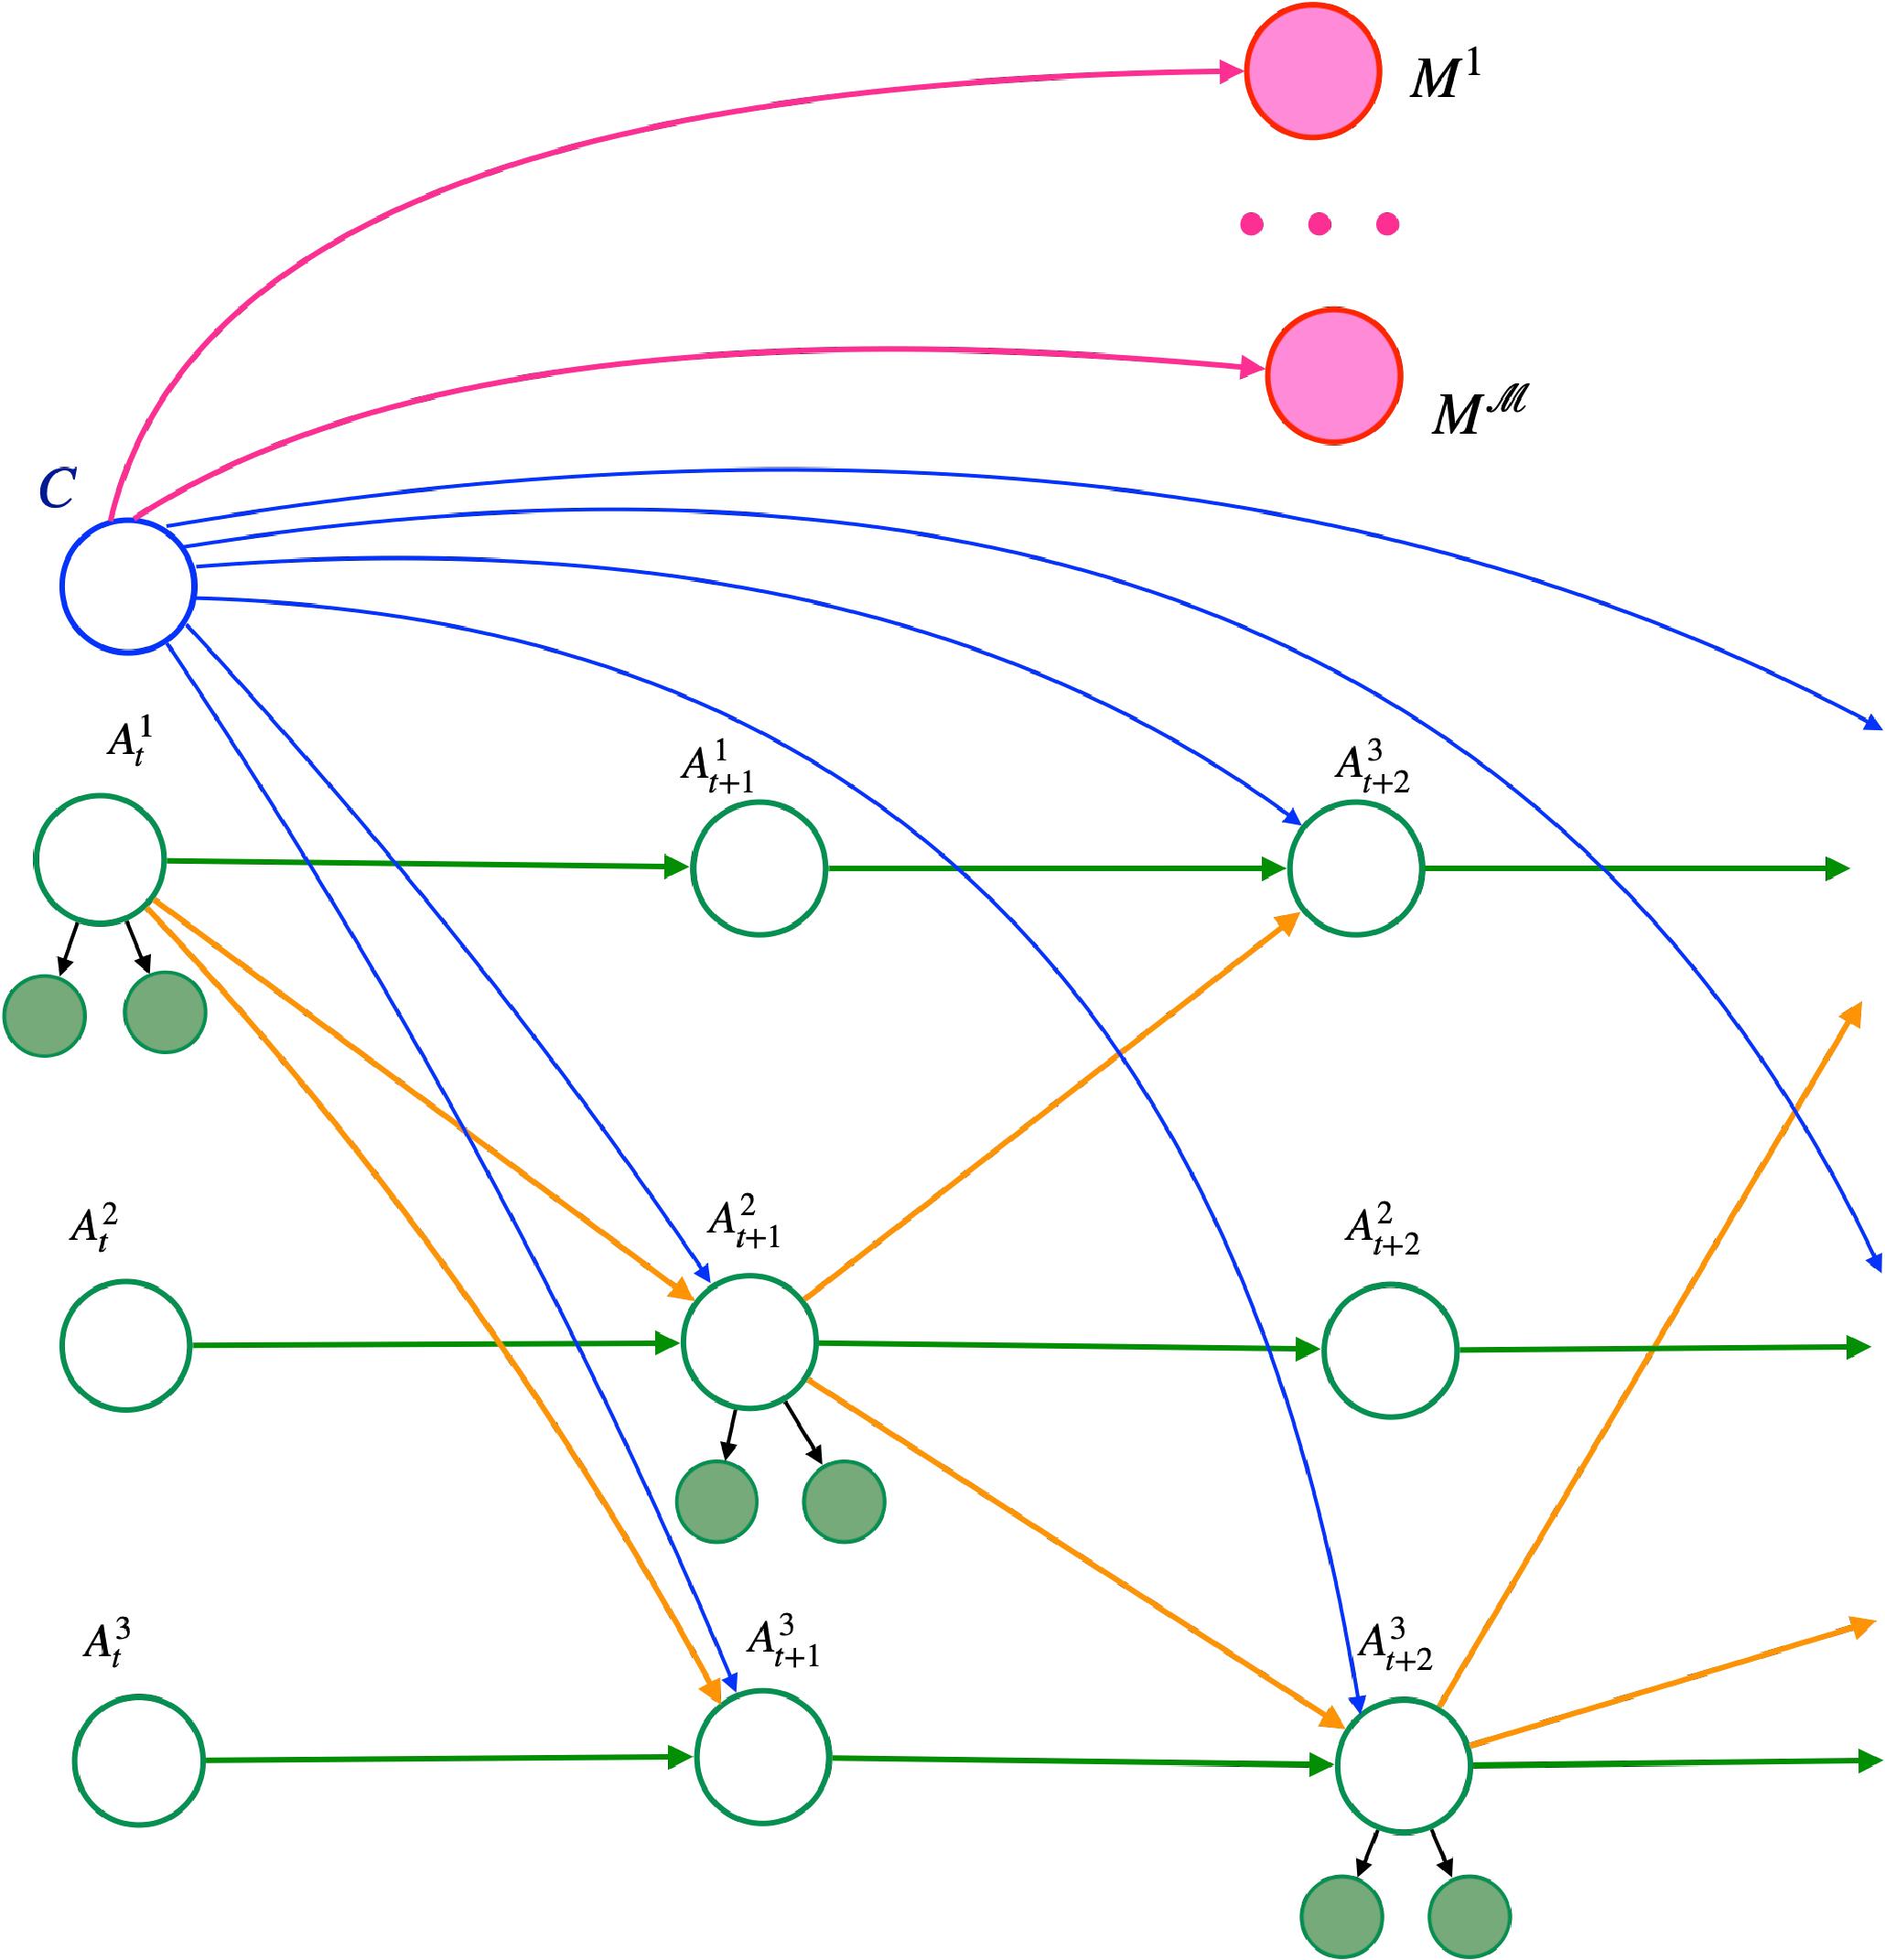
\includegraphics[width=\textwidth]{images/prereg-pgm.pdf}
        \caption{%
            Probabilistic graphical model (PGM) for investigating coordination.
            Circles (nodes) are stochastic variables.  Open circles are latent
            variables, shaded circles are potentially observed variables, and
            arrows represent variables conditioned on parents.  Coordination,
            $C$, is posited to influence team efficacy measures, $M^i$.  We do
            not use plate notation here because the conditioning arrows are
            measure specific). These are different linear functions learned
            from data with potentially different emission distributions (e.g.,
            normal or Poisson), depending on the measurement construct. \\
            $~~~~~~~~$ Coordination is exhibited by variables influencing other
            variables in the next time step. We do not draw all possible arrows
            here, because, for vocalics, we assume that all  such influence
            comes from the previous speaker.  Here we illustrate person 1
            speaking, followed by person 2, and then person 3.
        }
        \label{fig:pgm}
    \end{figure}
%
    The distributions $p(M^i|C)$ are typically linear functions learned from data
    with normal or Poisson emission distributions. Using a simple prior on $C$
    provides a baseline model.

    \paragraph{Coordination} We would like to study the effect of including
    coordination in this model.  We are developing a comprehensive
    probabilistic model for coordination, with a simple case exhibited as part
    of \autoref{fig:pgm}.  We will compare the predictive utility of that model
    with coordination to a simple baseline model without it.

    While in the general case coordination influences multiple diverse
    modalities at different time scales, here we consider a single time scale
    and two vocalic features.  Our underlying axiom is that higher coordination
    is associated with causally driven increased mutual information (statistical
    dependence) between relevant observed variables. Here we consider latent
    attributes for vocalic style for person $p$, denoted by $A^{p}$, which has
    as evidence, $O^{p,1}$, being the mean of normally distributed pitch of
    speech over a speech turn and similarly $O^{p,2}$ for speech intensity.  We
    further assume that the speech style of each person is only influenced by
    the previous speaker.

    If person 2 speaks after person 1, then the degree that their vocalic style
    follows that of person 1 indicates coordination. Formally, we blend the
    non-coordinated distribution mean, $\mu^2_t$, for the second person, with
    the fully dependent mean, $\mu^1_t$, for the mean for the second person at
    time $t+1$ by

    \begin{align}
        \mu^2_{t+1} = (1-c) \mu^2_t + c\mu^1_t ~.
    \end{align}

    To pre-register a single approach, we model coordination as being constant
    for the second half of each trial. This allows for the team to develop some
    rapport and interventions to have an effect. 

\subsection{Interventions}
\label{subsec:interventions}

The agent has a set of three interventions designed to encourage oral
communication among team members. The interventions are:

\begin{enumerate}

    \item \textbf{Marker Block:} the agent intervenes whenever a team member
        places a marker block but does not let their teammates know about it.

    \item \textbf{Help Request:} the agent intervenes whenever a team member
        needs assistance but does not ask for it.

    \item \textbf{Help-Request Reply:} the agent intervenes whenever a team
        member asks for help, but any of the other team members replies.

\end{enumerate}

The agent uses a state machine to determine when to watch/monitor, activate or
cancel a specific intervention. Different events in the game might trigger
different interventions and state transitions. The general idea is illustrated
in \autoref{fig:marker_block_intervention_flow_chart_general}.  The data comes
from different streams.  \autoref{tab:intervention_variables} contains a list
of topics the agent uses to gather relevant information about the missions.
The following subsections detail the specific events and rules associated with
each intervention the agent implements.

%
\begin{marginfigure}[-3.5in]
    \centering
    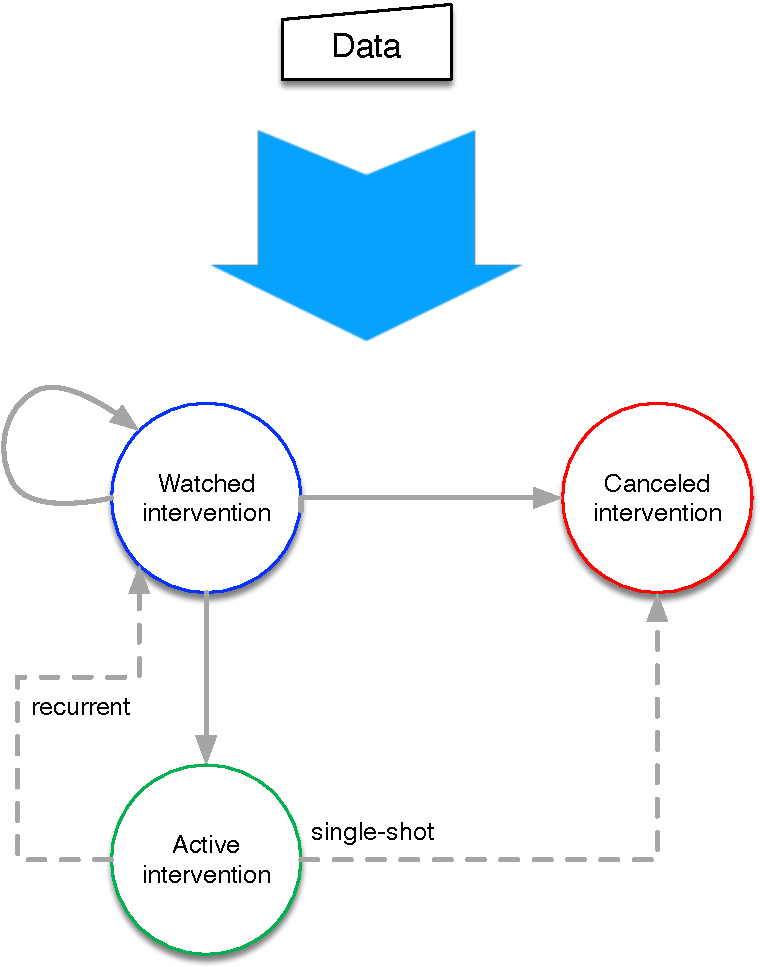
\includegraphics[width=\textwidth]{images/intervention_flow_chart_overview.pdf}
    \caption{%
        Intervention states and possible transitions. Based on specific events,
        the agent can start to watch a specific intervention at any moment.
        That intervention can either become active (delivered to particular
        team members) or canceled if it is no longer relevant. An active
        intervention can be watched again for possible reactivation (recurrent
        intervention), or it can be canceled if it needs to be delivered just a
        single time (single-shot intervention).
    }
    \label{fig:marker_block_intervention_flow_chart_general}
\end{marginfigure}

%
%
\begin{table}
    \small
    \centering
    \begin{tabularx}{6in}{lp{1.2in}X}
        \toprule
        Topic & Publisher & Purpose\\
        \midrule  
    	trial & simulator & Determine a mission start and end \\
    	observations/events/mission & simulator & Determine the list of team members and mission order \\    
    	agent/dialog & UAZ Dialog Agent & Determine relevant information from the team members' speech \\
    	observations/events/player/triage & simulator & Determine interaction with a victim \\    
    	observations/events/player/victim\_picked\_up & simulator & Determine interaction with a victim \\
    	observations/events/player/marker\_placed & simulator & Determine a marker placement \\
    	observations/events/player/marker\_removed & simulator & Determine a marker removal \\  
    	observations/state & simulator & Determine the team members' positions \\	
    	observations/events/player/role\_selected & simulator & Determine the team members' roles \\
    	observations/events/player/rubble\_collapse & simulator & Determine if an obstacle is blocking an exit \\
    	observations/events/player/tool\_used & simulator & Determine if an obstacle is being destroyed \\
    	observations/events/player/proximity & IHMC Proximity AC agent & Determine the team members' areas \\
    	observations/events/player/rubble\_destroyed & simulator & Determine an exit was unblocked \\   
    	agent/pygl\_fov/player/3d/summary & FoV Tool & Determine objects in the team members' field of view \\    	
        \bottomrule
    \end{tabularx}
    \caption{%
        List of testbed message topics the agent uses.
    }
    \label{tab:intervention_variables}
\end{table}
%


\subsubsection{Marker Block}

The agent will start to consider an intervention of this kind whenever a team
member places one of the following markers:

\begin{itemize}
	\item Critical Victim
	\item Regular Victim
	\item Rubble
	\item SOS
\end{itemize}

These markers communicate the need for assistance from other team members.
Thus, the team must ideally know when markers of these kinds are placed.
Although markers show up in the interactive map, the verbalization of a marker
placement ensures that team member actually pay attention to where the marker
is placed on the map, as they might miss the marker due to them not looking at
the map at the time of placement.  If the intervention is activated, the agent
will send the following message to the team member who placed the marker with the following
content:

\begin{quote} 
    \emph{``[Player color], let your teammates know about the [marker type]
    marker you recently placed."}
\end{quote}

The agent only intervenes once for each watched marker. This means that once
the intervention gets activated, the agent removes it from the queue of watched
interventions. The rules for switching to one state or another are detailed in
\autoref{fig:marker_block_intervention_flow_chart}.

%
\begin{figure}
    \centering
    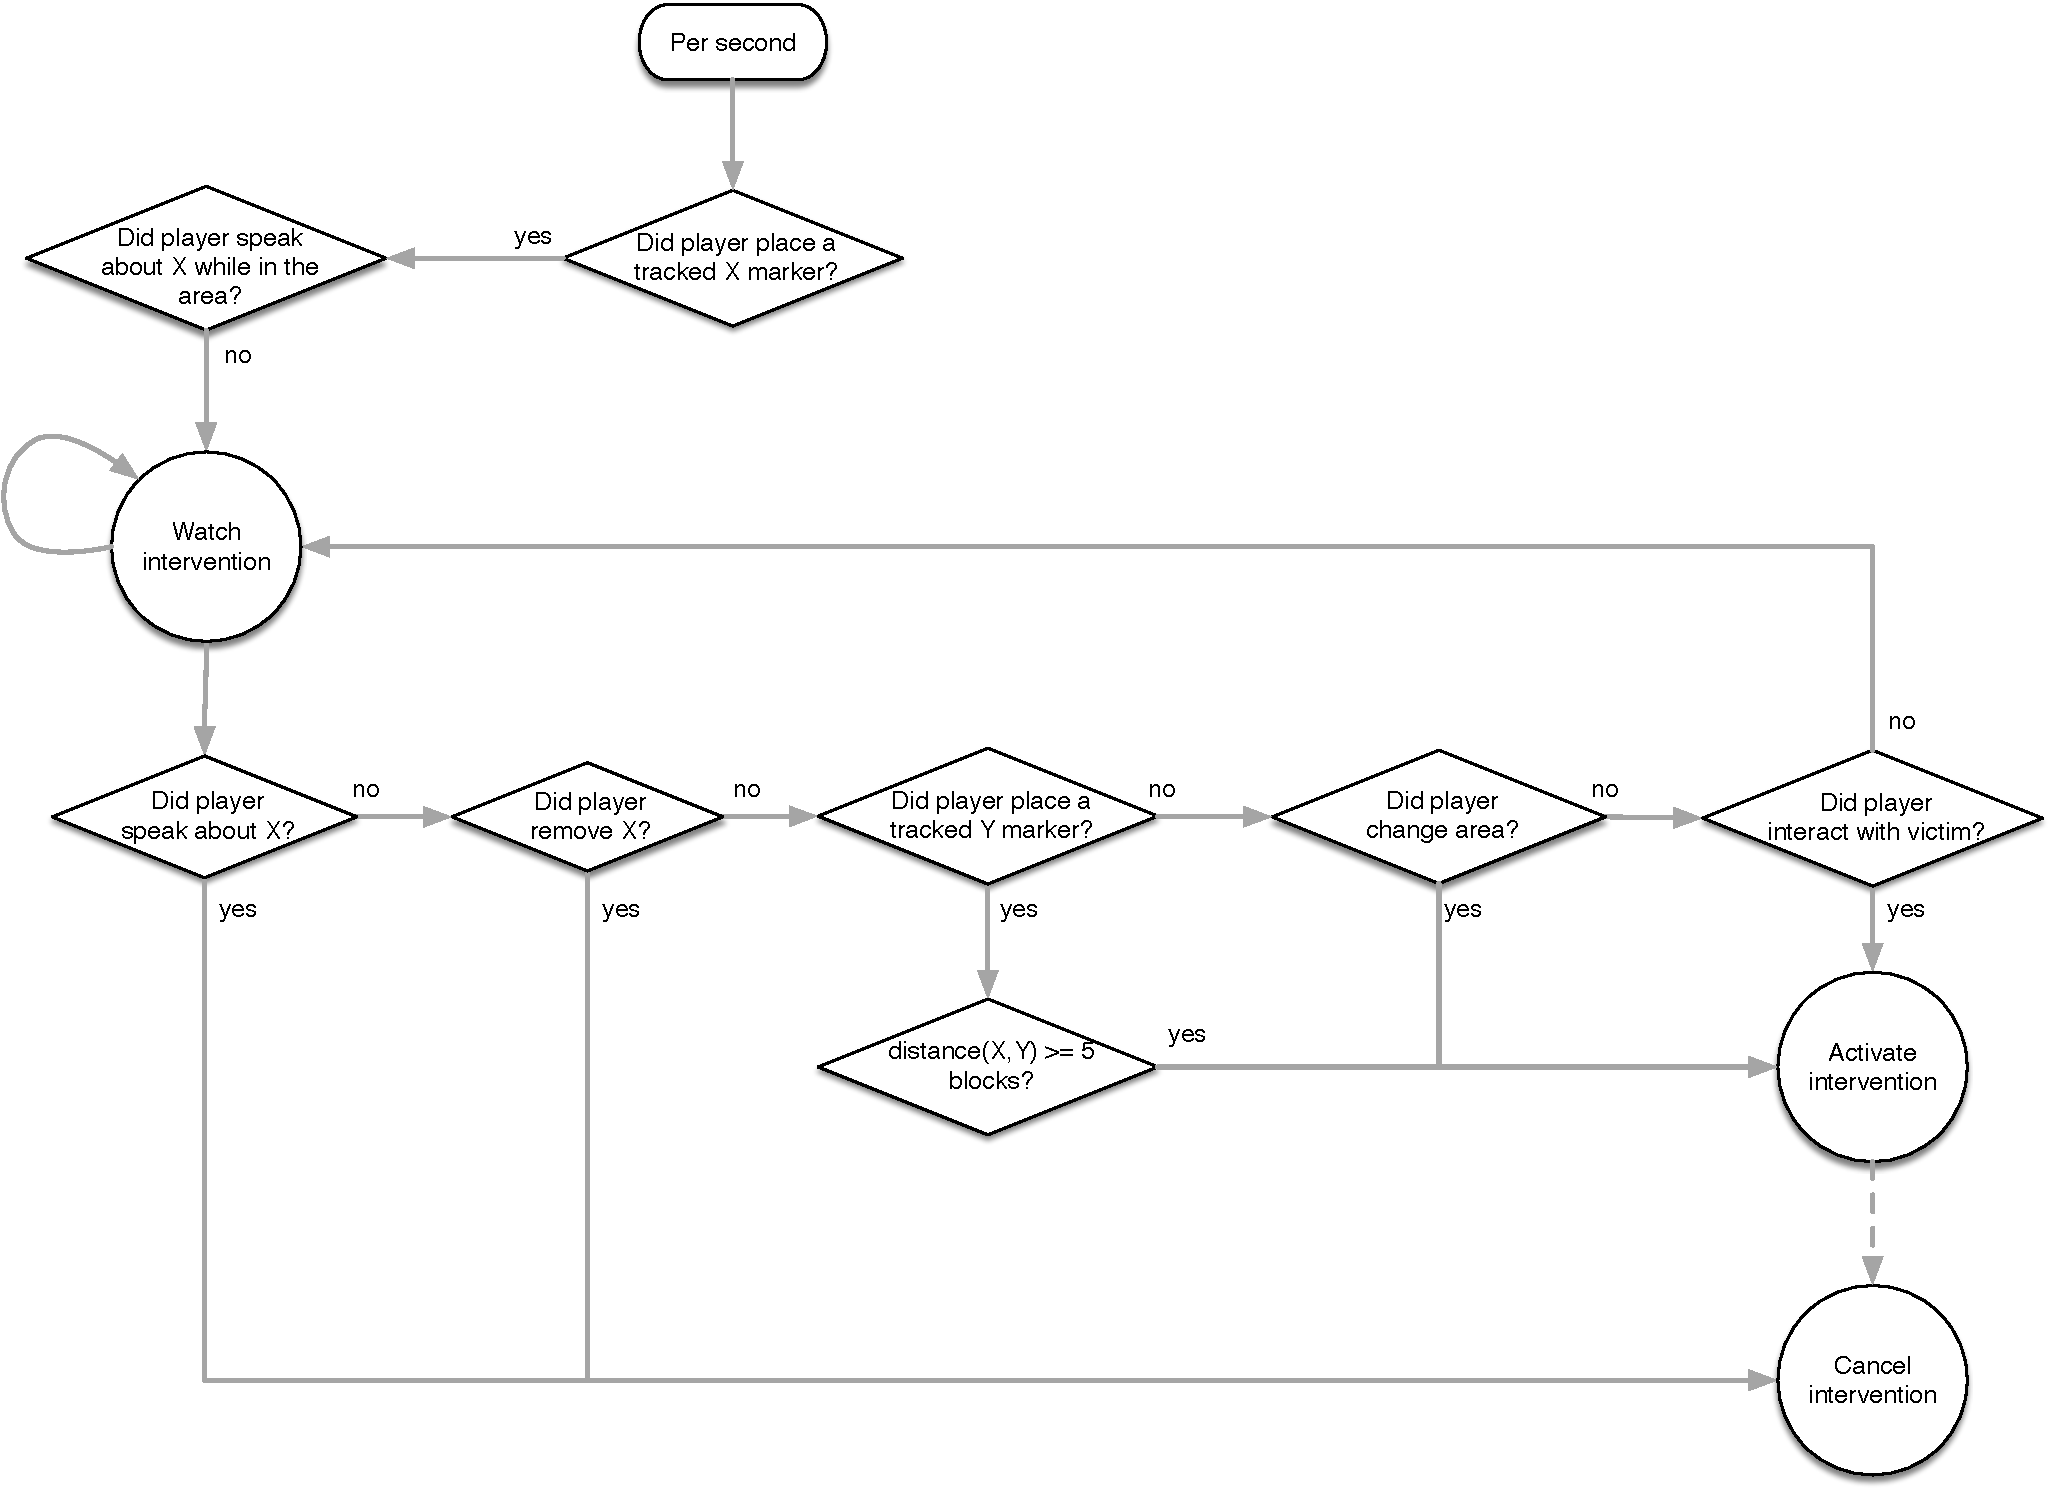
\includegraphics[width=\textwidth]{images/marker_block_intervention_flow_chart.pdf}
    \caption{%
        State transition rules for a marker-block intervention. The agent only
        intervenes once for each watched marker.This means that once the
        intervention gets activated, the agent removes it from the queue of
        watched interventions.
    }
    \label{fig:marker_block_intervention_flow_chart}
\end{figure}
%

\subsubsection{Help Request}

The agent will start to monitor for an intervention of this kind whenever a
team member notices they are trapped inside a threat room or when they are
close enough to a critical victim. These two events require team members to
request assistance from others.

The agent considers a team member to have noticed rubble blocking their way out
of a room if the obstructed exit is in the team member's field of view and
within five blocks of their position. The same rule is applied to determine
whether they perceived a critical victim or not. If the intervention is
activated, the agent will send one of the following messages to the team member
who needs help:

\begin{quote} 
    \emph{``[Player color], it seems you need some help to rescue a critical
    victim. Ask your teammates for assistance.''}
\end{quote}

\begin{quote} 
    \emph{``[Player color], it seems you need some help to exit this room. Ask
    your teammates for assistance.''}
\end{quote}

\noindent The rules for state transitions are illustrated in
\autoref{fig:help_request_intervention_flow_chart_re} and
\autoref{fig:help_request_intervention_flow_chart_cv}.

%
\begin{figure}
    \centering
    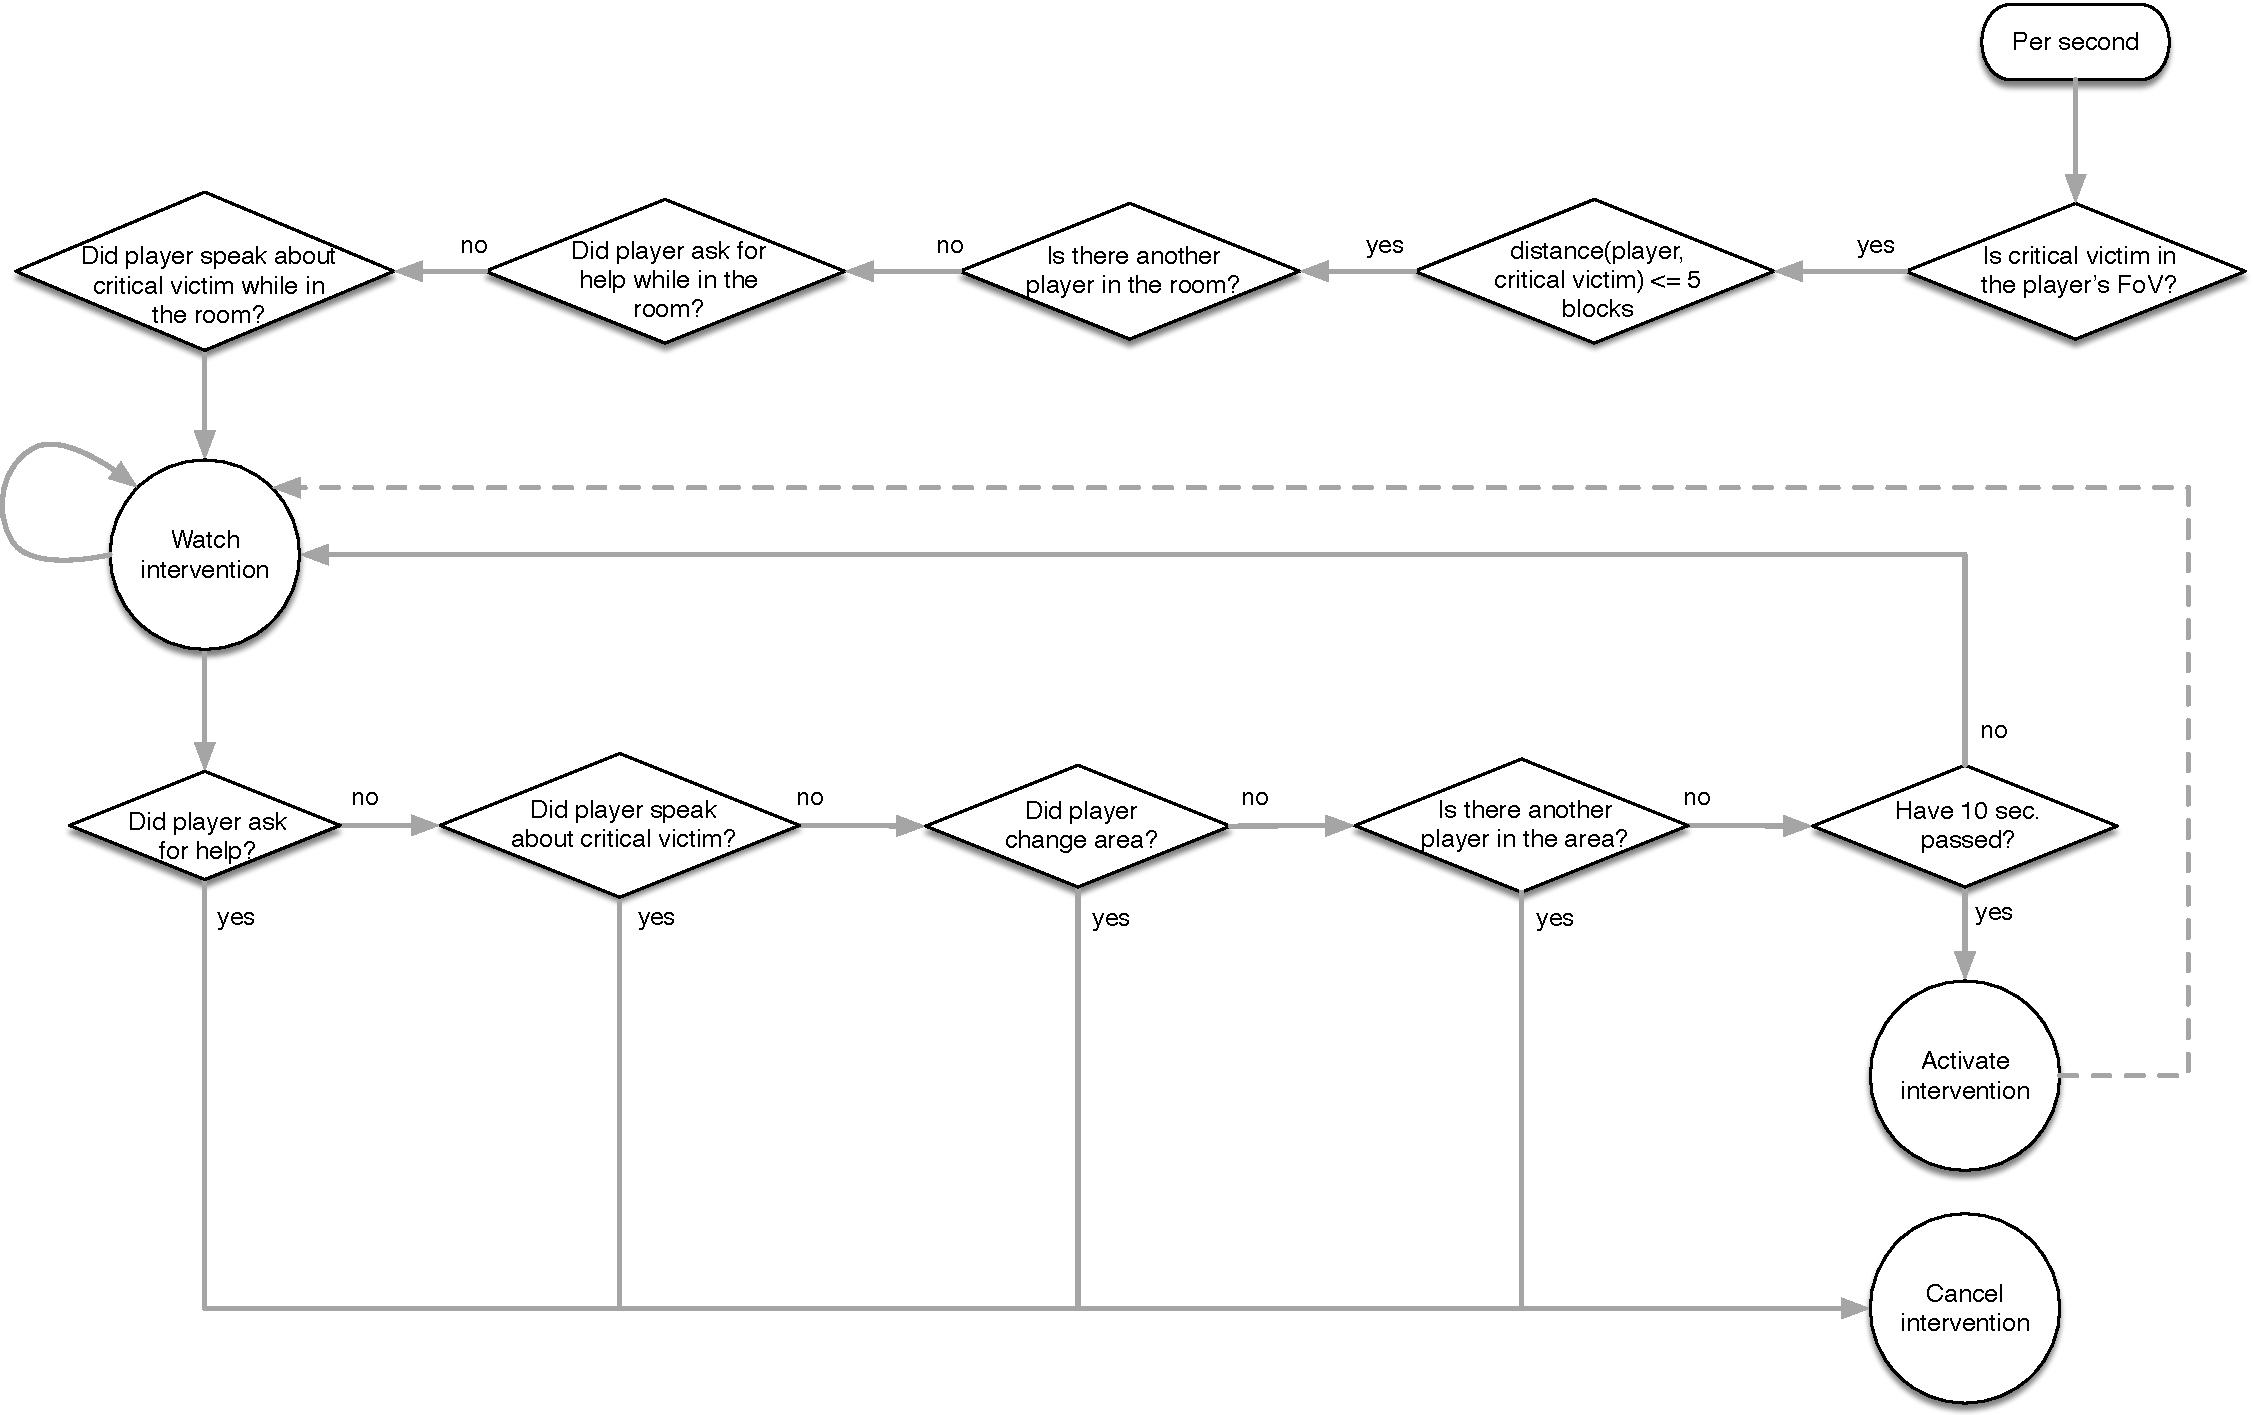
\includegraphics[width=\textwidth]{images/help_request_intervention_flow_chart_cv.pdf}
    \caption{%
        State transition rules for a help-request-for-critical-victim
        intervention. The agent can intervene multiple times if the objective
        of the intervention is not fulfilled. This means that once the
        intervention gets activated, the agent moves it back to the queue of
        watched interventions.
    }
    \label{fig:help_request_intervention_flow_chart_cv}
\end{figure}
%

%
\begin{figure}
    \centering
    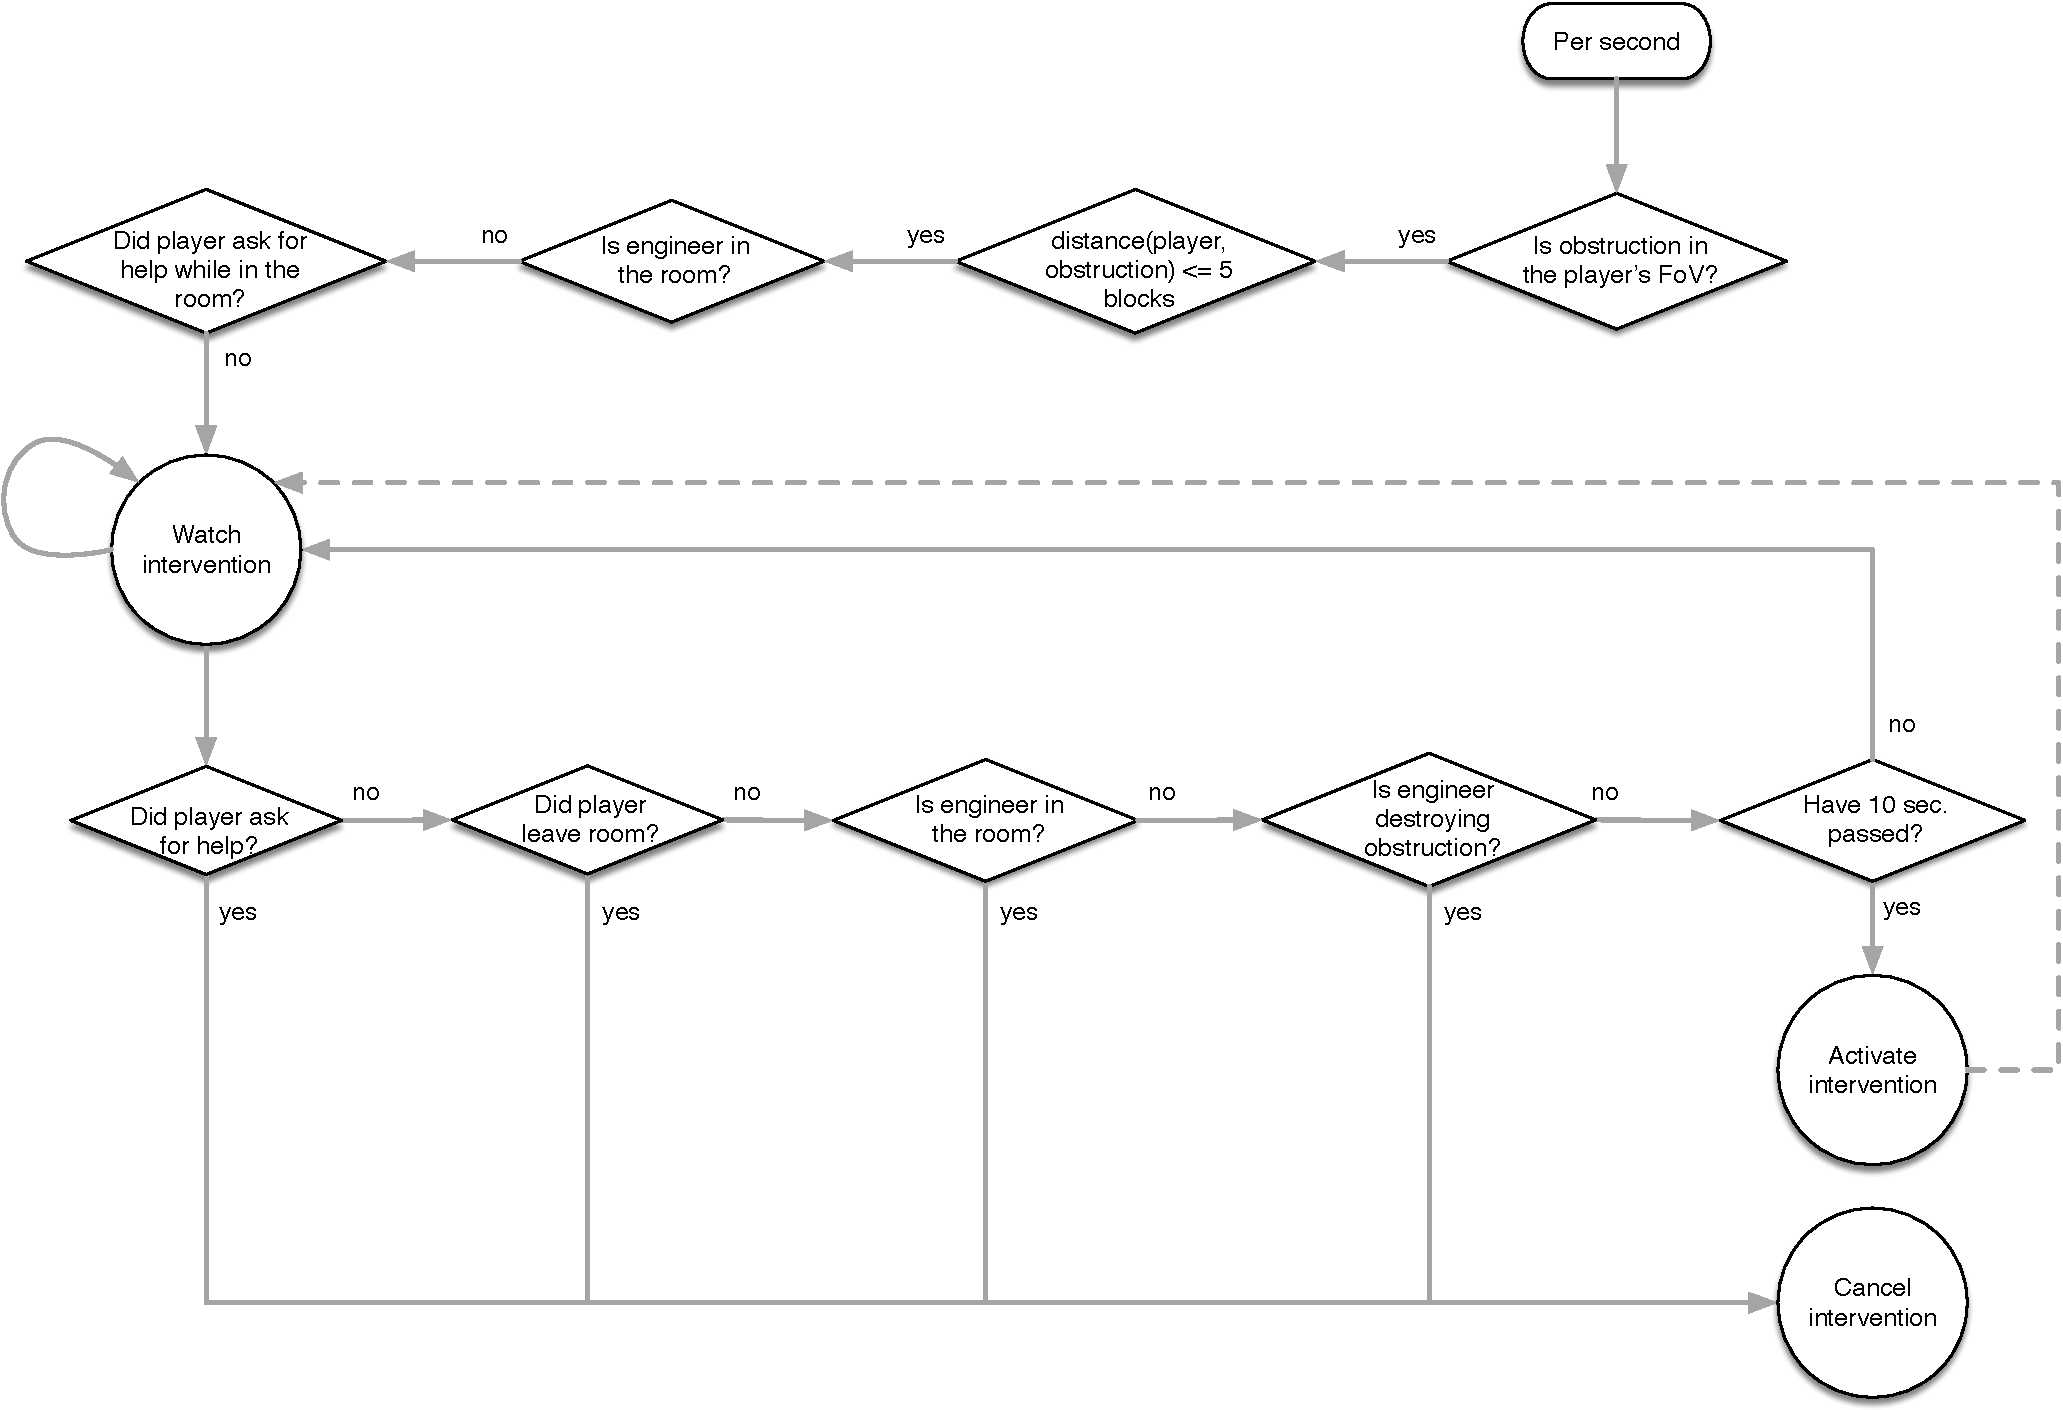
\includegraphics[width=\textwidth]{images/help_request_intervention_flow_chart_re.pdf}
    \caption{%
        State transition rules for a help-request-for-room-escape intervention.
        The agent can intervene multiple times if the objective of the
        intervention is not fulfilled. This means that once the intervention
        gets activated, the agent moves it back to the queue of watched
        interventions.
    }
    \label{fig:help_request_intervention_flow_chart_re}
\end{figure}
%

\subsubsection{Help Request Reply}

The agent will start to monitor for an intervention of this kind whenever a
team member asks for help. The agent uses the rule-based entity and event
extractions \ref{ch:rule_based_ie} to detect when a team member asks for help.
If the intervention is activated, the agent will send the following message to the team
member who asked for help:

\begin{quote} 
    \emph{``[Player color], it's been a while since you asked for help. Remind
    your teammates."}
\end{quote}

\noindent State transition rules are illustrated in
\autoref{fig:help_request_reply_intervention_flow_chart}.

%
\begin{figure}
    \centering
    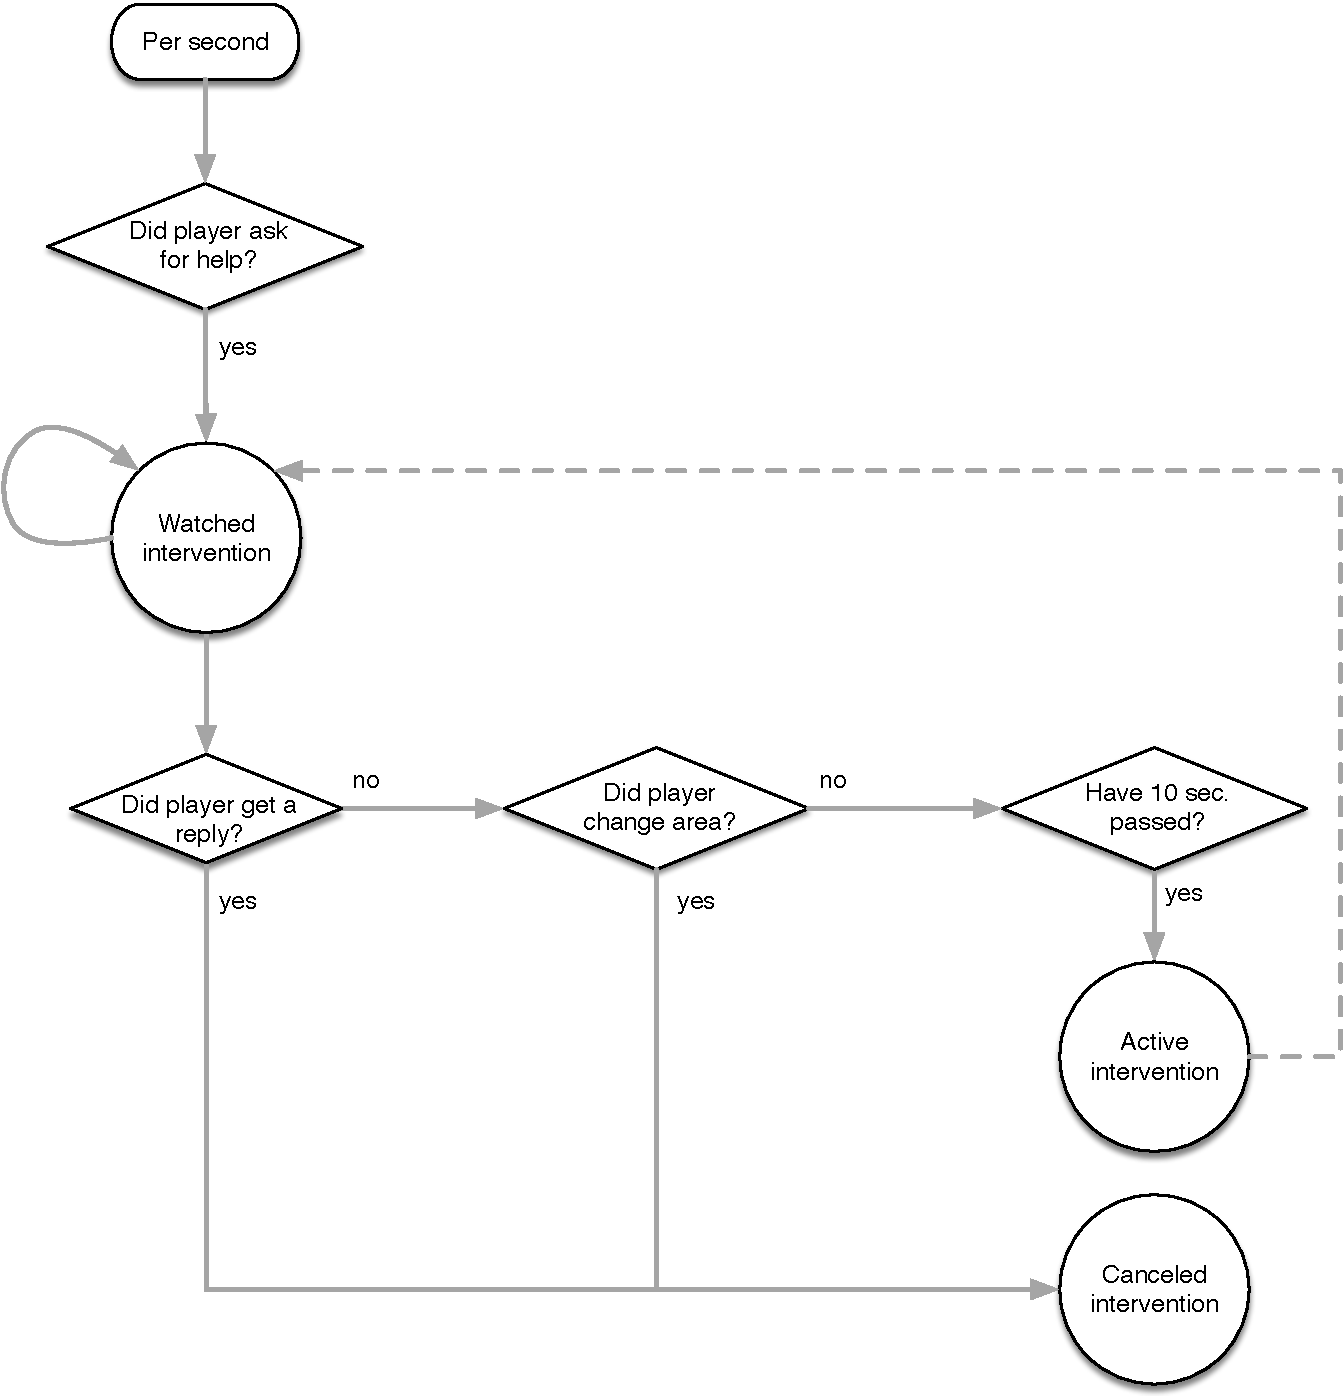
\includegraphics[width=\textwidth]{images/help_request_reply_intervention_flow_chart.pdf}
    \caption{%
        State transition rules for a help-request-for-room-escape intervention.
        The agent can intervene multiple times if the objective of the
        intervention is not fulfilled. This means that once the intervention
        gets activated, the agent moves it back to the queue of watched
        interventions.
    }
    \label{fig:help_request_reply_intervention_flow_chart}
\end{figure}
%

\section{Evaluation}

\textbf{Hypothesis 1: modeling coordination improves outcome prediction.}  For
hypothesis 1 we train two different models (with and without coordination) on
the same training sets in the cross validation splits. We then apply each model
to held out data. The result in either case is a distribution for each outcome
variable. Given the actual value of the outcome variable treated as a real
number, we will evaluate predictive accuracy by using the mean of the
distribution (MMSE loss) compared to the actual value, and compute the squared
error over all test splits in a leave one out cross validation scenario. For
completeness, for any categorical outcomes we would compare the value with
maximal probability (MAP loss) with the observed one. 

\noindent \textbf{Hypothesis 2: increased coordination predicts higher outcome measures.}
Here we are interested in the learned model, and cross-validation is not
critical, as the model is not trained on predicting higher outcome measures.  In
particular, we posit that the slopes in the sub-models for the measures, i.e.,
$p(M^i|C)$ will be positive. We will estimate the posterior distribution of
those slopes over relevant data. The mean and variance of that distribution will
give some idea as to the validity of the claim that coordination and a
particular measure are positively correlated.  Sampling this distribution will
reveal intervals that capture the probability that this is valid within various
ranges. 

\noindent \textbf{Hypothesis 3: intervening on team communication predicts higher
coordination and outcome measures.} Here we have two distinct data cases. Each
case leads to a probability distribution for coordination and outcome measures.
Specifically, each trial contributes multiple samples to one of those
distributions. We sample those distributions to evaluate the hypotheses within
the Bayesian hypothesis testing paradigm.  For each outcome measure we will
evaluate the probability that the claim is true for each outcome measure.
